\documentclass{article}
\usepackage{amsmath}
\usepackage{graphicx}
\usepackage{booktabs}

\title{K-Nearest-Neighbor en Python}
\author{[Carlos Oswaldo Gonzalez Garza]}


\begin{document}

\maketitle

\section{Introducci\'on}
K-Nearest-Neighbor es un algoritmo supervisado de Machine Learning que clasifica o predice datos según la similitud con ejemplos previos. Es fácil de implementar y se aplica en reconocimiento de patrones y sistemas de recomendación.
\section{Metodolog\'ia}
Se siguieron los siguientes pasos para realizar K-Nearest-Neighbor
\begin{enumerate}
    \item Primero hacemos imports de librerías que utilizaremos
    \begin{verbatim}
        import pandas as pd
        import numpy as np
        import matplotlib.pyplot as plt
        from matplotlib.colors import ListedColormap
        import matplotlib.patches as mpatches
        import seaborn as sb
        plt.show
        plt.rcParams['figure.figsize'] = (16, 9)
        plt.style.use('ggplot')
        from sklearn.model_selection import train_test_split
        from sklearn.preprocessing import MinMaxScaler
        from sklearn.metrics import classification_report
        from sklearn.metrics import confusion_matrix
    \end{verbatim}
    \item Cargamos el archivo entrada csv con pandas y aprovechamos a ver un resumen estadístico de los datos
    \begin{verbatim}
        dataframe = pd.read_csv(r"reviews_sentiment.csv",sep=';')
        print(dataframe.head(10))
        print(dataframe.describe())
    \end{verbatim}
    \item Veamos unas gráficas simples y qué información nos aportan
    \begin{verbatim}
        dataframe.hist()
        plt.show()
    \end{verbatim}
    \item Veamos realmente cuantas Valoraciones de Estrellas tenemos
    \begin{verbatim}
        print(dataframe.groupby('Star Rating').size())
    \end{verbatim}
    \item Hacemos otra grafica y tambien graficamos mejor la cantidad de palabras
    \begin{verbatim}
        sb.catplot(x='Star Rating',data=dataframe,kind="count", aspect=3)
        sb.catplot(x='wordcount',data=dataframe,kind="count", aspect=3)
        plt.show()
    \end{verbatim}
    \item Creamos nuestro X e y de entrada y los sets de entrenamiento y test.
    \begin{verbatim}
        X = dataframe[['wordcount','sentimentValue']].values
        y = dataframe['Star Rating'].values

        X_train, X_test, y_train, y_test = train_test_split(X, y, random_state=0)
        scaler = MinMaxScaler()
        X_train = scaler.fit_transform(X_train)
        X_test = scaler.transform(X_test)
    \end{verbatim}    
    \item Definimos el valor de k en 7 y creamos nuestro clasificador.
    \begin{verbatim}
        n_neighbors = 7

        knn = KNeighborsClassifier(n_neighbors)
        knn.fit(X_train, y_train)
        print('Accuracy of K-NN classifier on training set: {:.2f}'
        .format(knn.score(X_train, y_train)))
        print('Accuracy of K-NN classifier on test set: {:.2f}'
        .format(knn.score(X_test, y_test)))
    \end{verbatim}
    \item Precisión del modelo
    \begin{verbatim}
        pred = knn.predict(X_test)
        print(confusion_matrix(y_test, pred))
        print(classification_report(y_test, pred))
    \end{verbatim}
    \item Y graficamos.
    \begin{verbatim}
        h = .02 # step size in the mesh

        # Create color maps
        cmap_light = ListedColormap(['#FFAAAA', '#ffcc99', '#ffffb3','#b3ffff',
        '#c2f0c2'])
        cmap_bold = ListedColormap(['#FF0000', '#ff9933','#FFFF00','#00ffff',
        '#00FF00'])

        # we create an instance of Neighbours Classifier and fit the data.
        clf = KNeighborsClassifier(n_neighbors, weights='distance')
        clf.fit(X, y)

        # Plot the decision boundary. For that, we will assign a color to each
        # point in the mesh [x_min, x_max]x[y_min, y_max].

        x_min, x_max = X[:, 0].min() - 1, X[:, 0].max() + 1
        y_min, y_max = X[:, 1].min() - 1, X[:, 1].max() + 1
        xx, yy = np.meshgrid(np.arange(x_min, x_max, h),
        np.arange(y_min, y_max, h))
        Z = clf.predict(np.c_[xx.ravel(), yy.ravel()])

        # Put the result into a color plot
        Z = Z.reshape(xx.shape)
        plt.figure()
        plt.pcolormesh(xx, yy, Z, cmap=cmap_light)

        # Plot also the training points
        plt.scatter(X[:, 0], X[:, 1], c=y, cmap=cmap_bold,edgecolor='k', s=20)
        plt.xlim(xx.min(), xx.max())
        plt.ylim(yy.min(), yy.max())
        patch0 = mpatches.Patch(color='#FF0000', label='1')
        patch1 = mpatches.Patch(color='#ff9933', label='2')
        patch2 = mpatches.Patch(color='#FFFF00', label='3')
        patch3 = mpatches.Patch(color='#00ffff', label='4')
        patch4 = mpatches.Patch(color='#00FF00', label='5')
        plt.legend(handles=[patch0, patch1, patch2, patch3,patch4])

        plt.title("5-Class classification (k = %i, weights = '%s')"
        % (n_neighbors, 'distance'))

        plt.show()
    \end{verbatim}
    \item Elegimos el mejor valor de k
    \begin{verbatim}
        plt.show()
        k_range = range(1, 20)
        scores = []
        for k in k_range:
            knn = KNeighborsClassifier(n_neighbors = k)
        knn.fit(X_train, y_train)
        scores.append(knn.score(X_test, y_test))
        plt.figure()
        plt.xlabel('k')
        plt.ylabel('accuracy')
        plt.scatter(k_range, scores)
        plt.xticks([0,5,10,15,20])
    \end{verbatim}
    \item Predecir nuevas muestras
    \begin{verbatim}
        print(clf.predict([[5, 1.0]]))
        print(clf.predict_proba([[20, 0.0]]))
    \end{verbatim}
\end{enumerate}

\subsection{C\'odigo en Python}
\begin{verbatim}
    import pandas as pd
    import numpy as np
    import matplotlib.pyplot as plt
    from matplotlib.colors import ListedColormap
    import matplotlib.patches as mpatches
    import seaborn as sb
    plt.show
    plt.rcParams['figure.figsize'] = (16, 9)
    plt.style.use('ggplot')
    from sklearn.model_selection import train_test_split
    from sklearn.preprocessing import MinMaxScaler
    from sklearn.neighbors import KNeighborsClassifier
    from sklearn.metrics import classification_report
    from sklearn.metrics import confusion_matrix
    dataframe = pd.read_csv(r"reviews_sentiment.csv",sep=';')
    print(dataframe.head(10))
    print(dataframe.describe())
    dataframe.hist()
    plt.show()
    print(dataframe.groupby('Star Rating').size())
    sb.catplot(x='Star Rating',data=dataframe,kind="count", aspect=3)
    sb.catplot(x='wordcount',data=dataframe,kind="count", aspect=3)
    plt.show()
    X = dataframe[['wordcount','sentimentValue']].values
    y = dataframe['Star Rating'].values
    
    X_train, X_test, y_train, y_test = train_test_split(X, y, random_state=0)
    scaler = MinMaxScaler()
    X_train = scaler.fit_transform(X_train)
    X_test = scaler.transform(X_test)
    n_neighbors = 7
    
    knn = KNeighborsClassifier(n_neighbors)
    knn.fit(X_train, y_train)
    print('Accuracy of K-NN classifier on training set: {:.2f}'
    .format(knn.score(X_train, y_train)))
    print('Accuracy of K-NN classifier on test set: {:.2f}'
    .format(knn.score(X_test, y_test)))
    pred = knn.predict(X_test)
    print(confusion_matrix(y_test, pred))
    print(classification_report(y_test, pred))
    h = .02 # step size in the mesh
    
    # Create color maps
    cmap_light = ListedColormap(['#FFAAAA', '#ffcc99', '#ffffb3','#b3ffff','#c2f0c2'])
    cmap_bold = ListedColormap(['#FF0000', '#ff9933','#FFFF00','#00ffff','#00FF00'])
    
    # we create an instance of Neighbours Classifier and fit the data.
    clf = KNeighborsClassifier(n_neighbors, weights='distance')
    clf.fit(X, y)
    
    # Plot the decision boundary. For that, we will assign a color to each
    # point in the mesh [x_min, x_max]x[y_min, y_max].
    
    x_min, x_max = X[:, 0].min() - 1, X[:, 0].max() + 1
    y_min, y_max = X[:, 1].min() - 1, X[:, 1].max() + 1
    xx, yy = np.meshgrid(np.arange(x_min, x_max, h),
    np.arange(y_min, y_max, h))
    Z = clf.predict(np.c_[xx.ravel(), yy.ravel()])
    
    # Put the result into a color plot
    Z = Z.reshape(xx.shape)
    plt.figure()
    plt.pcolormesh(xx, yy, Z, cmap=cmap_light)
    
    # Plot also the training points
    plt.scatter(X[:, 0], X[:, 1], c=y, cmap=cmap_bold,edgecolor='k', s=20)
    plt.xlim(xx.min(), xx.max())
    plt.ylim(yy.min(), yy.max())
    patch0 = mpatches.Patch(color='#FF0000', label='1')
    patch1 = mpatches.Patch(color='#ff9933', label='2')
    patch2 = mpatches.Patch(color='#FFFF00', label='3')
    patch3 = mpatches.Patch(color='#00ffff', label='4')
    patch4 = mpatches.Patch(color='#00FF00', label='5')
    plt.legend(handles=[patch0, patch1, patch2, patch3,patch4])
    
    plt.title("5-Class classification (k = %i, weights = '%s')"
    % (n_neighbors, 'distance'))
    
    plt.show()
    k_range = range(1, 20)
    scores = []
    for k in k_range:
        knn = KNeighborsClassifier(n_neighbors = k)
    knn.fit(X_train, y_train)
    scores.append(knn.score(X_test, y_test))
    plt.figure()
    plt.xlabel('k')
    plt.ylabel('accuracy')
    plt.scatter(k_range, scores)
    plt.xticks([0,5,10,15,20])
    print(clf.predict([[5, 1.0]]))
    print(clf.predict_proba([[20, 0.0]]))
\end{verbatim}

\section{Resultados}
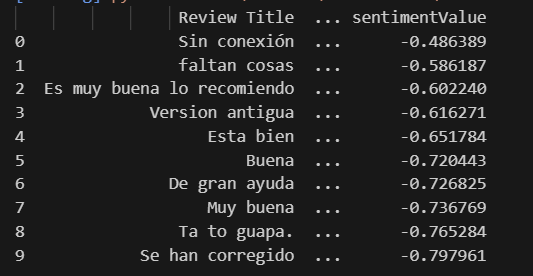
\includegraphics[width=12cm, height=6cm]{tabla1.png} 
\\
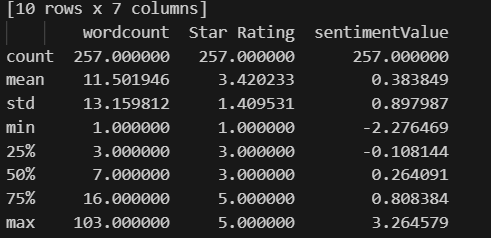
\includegraphics[width=12cm, height=6cm]{tabla2.png} 
\\
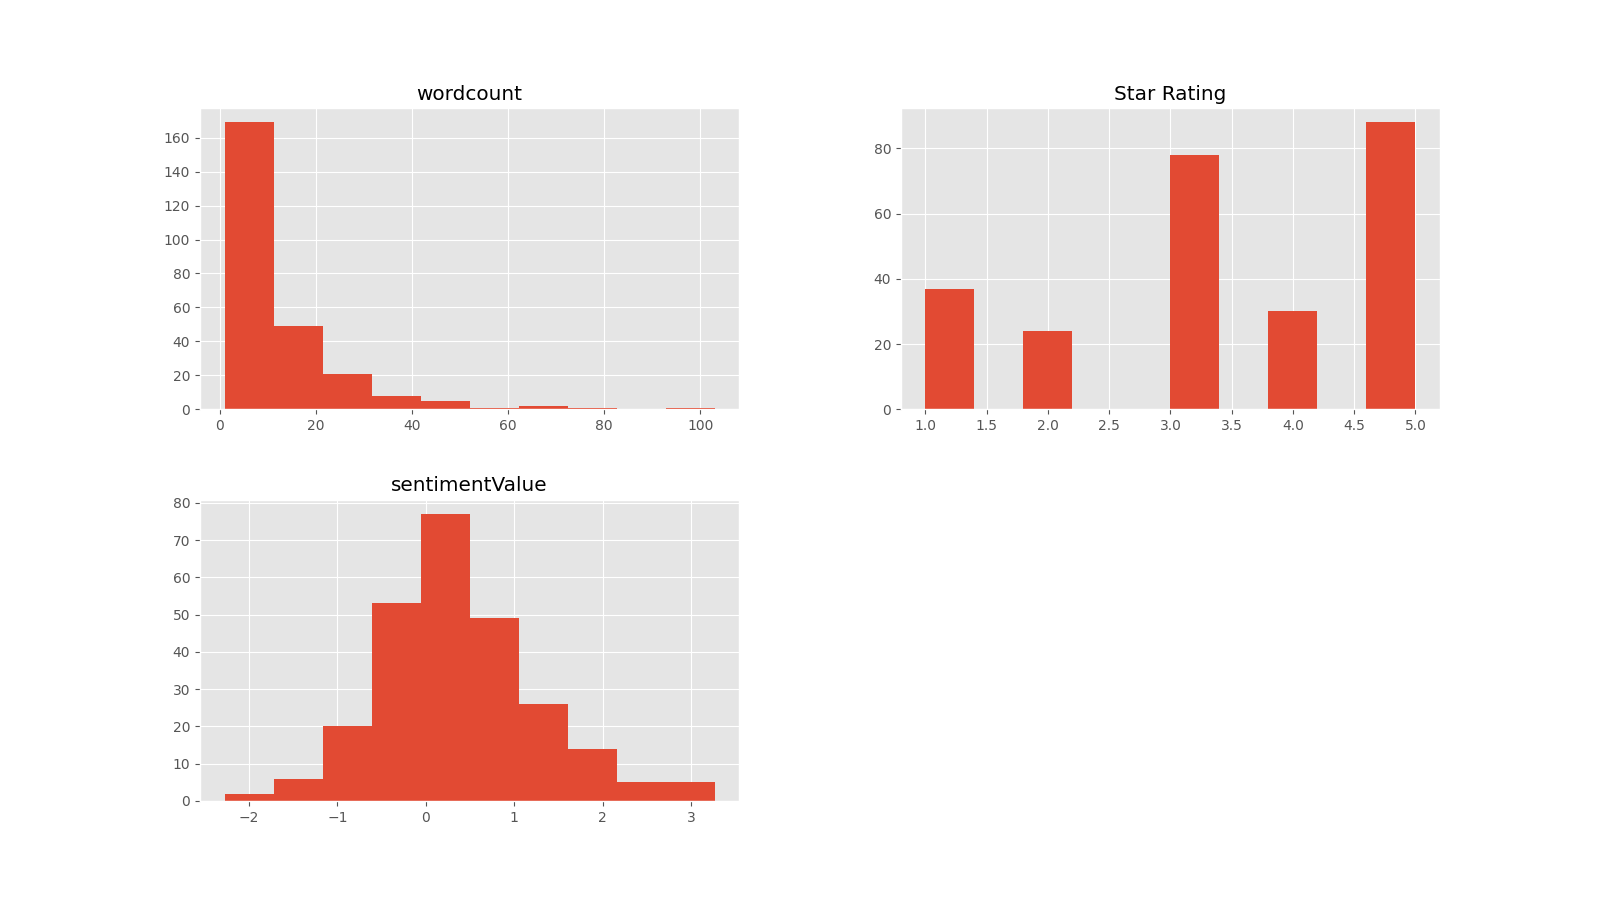
\includegraphics[width=14cm, height=8cm]{Figure_1.png} 
\\
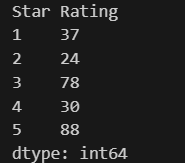
\includegraphics[width=5cm, height=3cm]{tabla3.png} 
\\
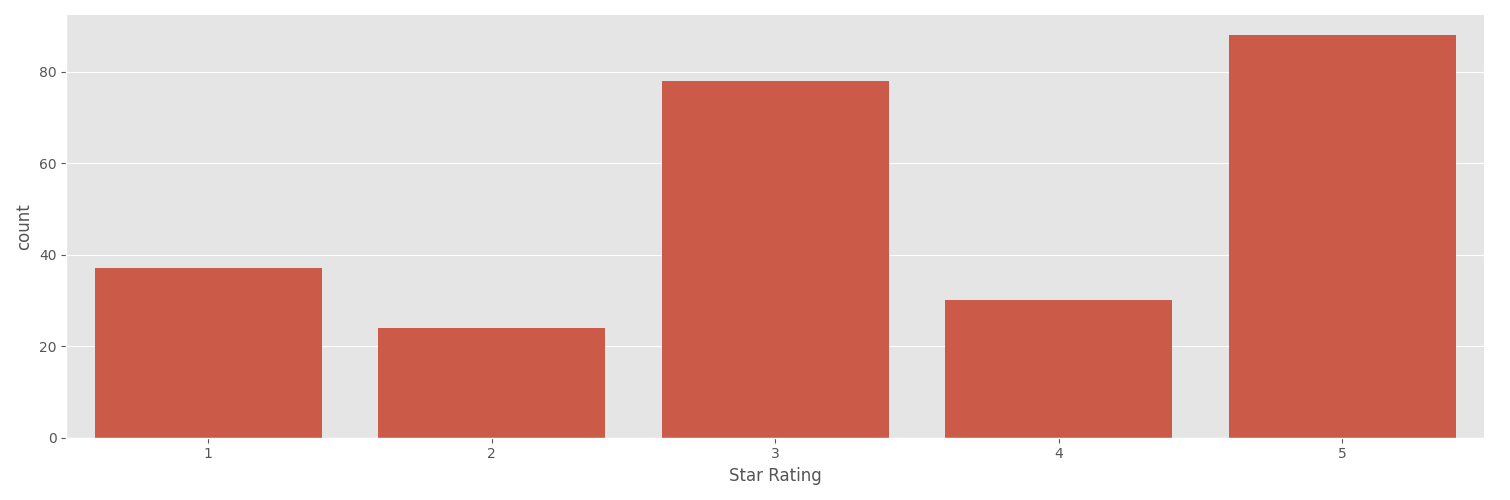
\includegraphics[width=14cm, height=8cm]{Figure_3.png} 
\\
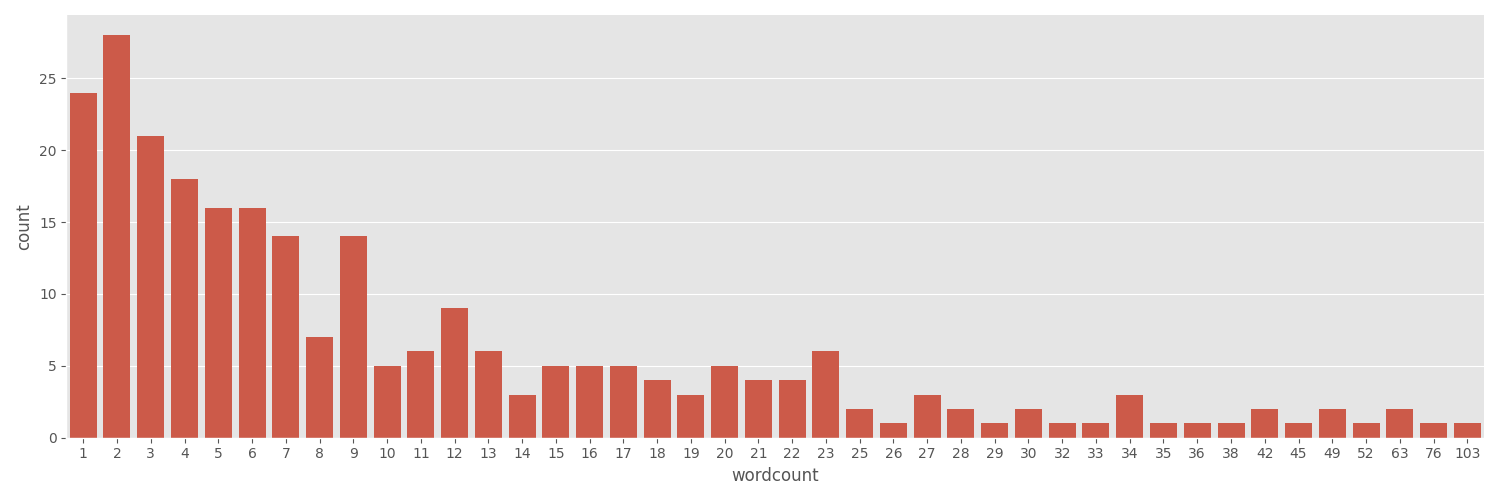
\includegraphics[width=15cm, height=8cm]{Figure_2.png} 
\\
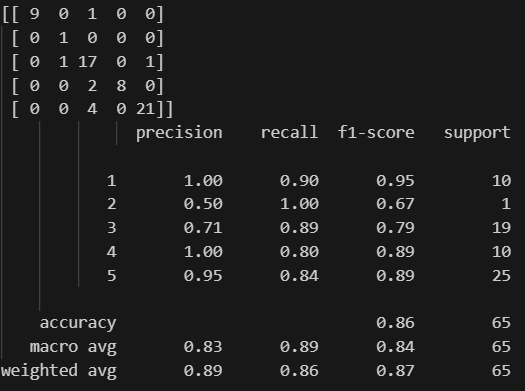
\includegraphics[width=14cm, height=8cm]{tabla4.png} 
\\
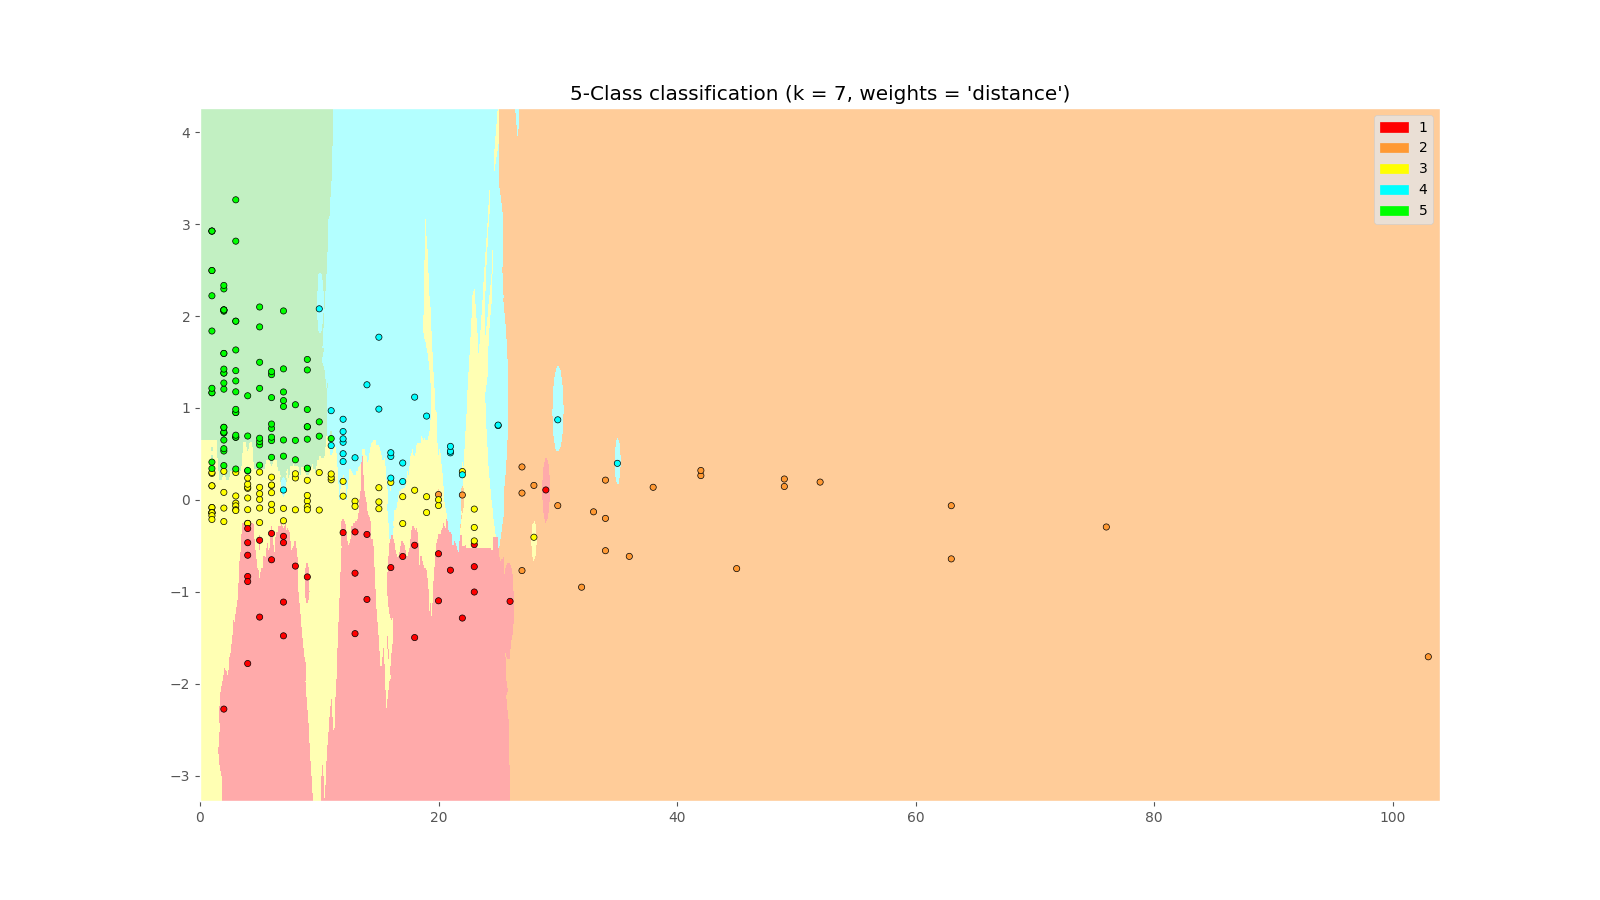
\includegraphics[width=14cm, height=8cm]{Figure_4.png} 
\\
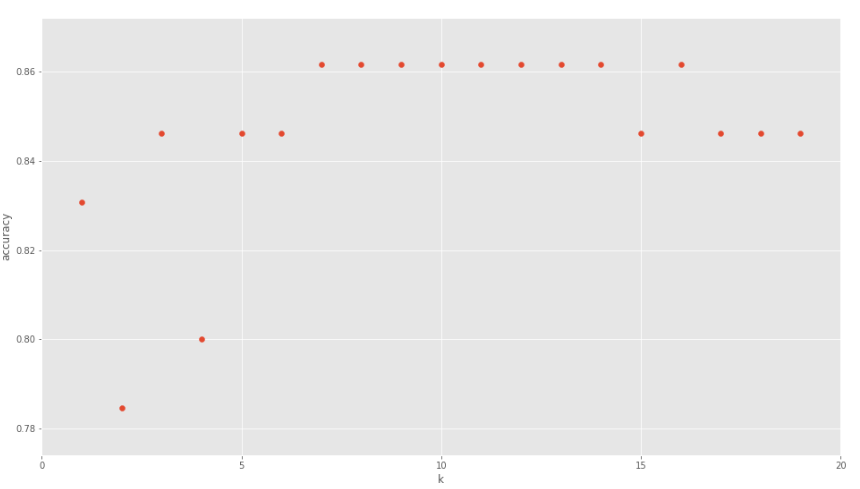
\includegraphics[width=14cm, height=8cm]{Figure_5.png} 
\begin{verbatim}
    ccuracy of K-NN classifier on training set: 0.90
    Accuracy of K-NN classifier on test set: 0.86
    [5]
    [[0.00381998 0.02520212 0.97097789 0. 0. ]]
\end{verbatim}

\section{Conclusi\'on}
En este ejercicio creamos un modelo en Python con K-Nearest Neighbor para clasificar puntos según sus "k vecinos más cercanos". Como es un algoritmo supervisado, requiere suficientes datos etiquetados para entrenarse. Aunque es simple, consume mucha memoria y CPU, por lo que no es ideal para grandes datasets. Usamos solo dos dimensiones para visualizar los grupos y realizar predicciones, lo que ayudó a comprender mejor el problema.
\end{document}